
% -*- TeX-master: "../dipole_ilya_paper.tex" -*-
\section{Operations with qubits}
\label{sec:characterisation}

% \red{Need scattering data}

\noindent  We record  the energy  spectrum  of the  twin qubit  using a  network
analyzer,  while  sweeping  the  biasing  magnetic flux.   Because  of  a  small
asymmetry, $\eta$, the fluxes linked through  the left and right loops are slightly
different: $ \Phi = \frac{\varphi}{2\pi}\Phi_0$ and $ \eta\Phi $, where $\eta\approx1$.

The  \iket{1}~\ilra~\iket{2}  transition, $\omega_{21}$,  is  mapped  with a  network
analyzer which measures  the transmission of signal  $\omega_{\text{NA}}$ through the
system.  Away from  resonance the signal passes through the  circuit without any
interaction with the qubit.  After  correcting for the line losses, transmission
is close to  $ 100\% $.  Only near resonance  ($\omega_{\text{NA}}=\omega_{21}$), does the
qubit exchange photons  with the driving field as it  evolves between the ground
and excited states.  The  qubit emits a wave that is  exactly in anti-phase with
the driving  field \cite{abdumalikov2010}, and the  destructive superposition in
the output line results in  a transmission dip, see Fig.~\ref{fig:transmission}.
The trace of blue circles of  the transmission minima at different magnetic flux
maps   out   the   qubit's   $\omega_{21}$  transition   spectrum,   see   inset   of
Fig.~\ref{fig:transmission}.

\begin{figure}[h]
  \centering\def\svgwidth{9.5cm}\import{images_inkscape/}{fig2.pdf_tex}
  \caption{\small \textbf{Mapping  the qubit transition  spectrum:}  For the  lower transition
    $\omega_{21}$ (blue) a  network analyzer measures  the power  transmission coefficient,
    \iabsSquared{t}, at flux  bias $ \Phi $  and microwave frequency $  \omega_{21}/2\pi$.  A Lorentzian
    fit \cite{Astafiev2010}  to the transmission  profile establishes the  resonant frequency,
    which  is  marked  with  blue  points on  the  flux-frequency  spectrum.   For  transition
    $\omega_{32}$  (red)  a two-tone  measurement is  run by  monitoring changes  to a  weak
    $\omega_{21}$ probe while sweeping a second frequency  in search of the higher transition.
    % Any changes to the probe's transmission are indicative of hitting the higher transition, which
    % is marked with a red point on the spectrum.
    % Readings are taken about the degeneracy point
    % $  \Phi \sim  \Phi_{0}/2 $,  where the  low  curvature of  transition energies,  allows for  stable
    % measurements with respect to fluctuations in the field.
  }
  \label{fig:transmission}
\end{figure}

The  \iket{2}\ilra\iket{3}  transition,  $\omega_{32}$,   is  mapped  using  two-tone
spectroscopy.   The network  analyzer probes  signals at  $ \omega_{21}  $, while  an
additional generator  sweeps a second  frequency, $ \omega_{\text{GEN}}  $.  Whenever
the      generator     strikes      the     \iket{2}\ira\iket{3}      transition
($\omega_{\text{GEN}}  = \omega_{32}  $), the  qubit  undergoes a  ladder of  excitations,
\iket{1}  \iratext{$\omega_{21}$}\iket{2}  \iratext{$\omega_{32}$} \iket{3},  depopulating
states \iket{1} and \iket{2}.  Because of this depopulation, the probe signal is
no longer  absorbed to drive  the \iket{1}\ilra \iket{2} transmission,  and it's
transmission  moves out  of  the resonance  dip in  Fig.~\ref{fig:transmission}.
This identifies  $\omega_{32}$ which  is mapped  with red  circles in  the transition
energy-magnetic field spectrum.

% prove that state 1 becomes depopulated  by solving the master equation for two
% drives

We match the  experimental data points to simulations: Islands,  isolated by the
JJ  in  Fig.~\ref{fig:setup},  are  labeled with  Cooper  pair  (CP)  occupation
$       \vec{n}      =       \iket{n_1,      n_2,       n_3}      $,       phase
$     \vec{\varphi}     =     \iket{\varphi_1,     \varphi_2,     \varphi_3}     $     and     potential
$ \vec{V} = \iket{V_{1}, V_{2}, V_{3}}  $ states.  The charges and potentials on
the islands are linked by the capacitance matrix
\begin{equation}
  \label{eq:link}
  2e\vec{n} = \hat{C}\vec{V}.
\end{equation}

\noindent The capacitance matrix in the twin qubit topology is
\begin{equation}
  \label{eq:capac}
  \hat{C} = \iabs{C} \begin{pmatrix}
    2  &  -1  &  0\\
    -1  &  2  +  \alpha  &  -1\\
    0  &  -1  & 2
  \end{pmatrix},
\end{equation}

\noindent where \iabs{C}  is the capacitance of the outer  JJs.  The interaction
of the  CPs, carrying a  charge $ \vec{Q}=2e\vec{n}  $, and potentials  on their
respective islands gives rise to the `kinetic' term of the Hamiltonian:
\begin{equation}\label{eq:kinetic}
  \begin{aligned}
    T = \frac{1}{2}\sum_{i=1}^{3}Q_iV_i & =
    \frac{(2e)^2}{2}\vec{n}\hat{C}^{-1}\vec{n}^{T}\\
    & = E_C \iabs{C} \iaverage{\hat{C}^{-1}}_{\iket{n_{1}, n_2, n_3}},
  \end{aligned}
\end{equation}

\noindent where we define $ E_{C}={(2e)^{2}}/{2 \iabs{C} } $.

Each  JJ  with  a  phase  difference  of  $\Delta\varphi_{i}$,  contributes  an  energy  of
$ E_{Ji}\left(1 - \cos(\Delta\varphi_i)\right) $.   The flux quantization condition for the
left                     and                    right                     loops,
$ \sum_{i}^{\text{loop}}  \varphi_i = 2\pi  n, n \in \mathbb{Z}$,  enters as a  dependence on
$ \varphi_\text{ext} $ and $ \eta\varphi_\text{ext} $ on two of the junctions:
\begin{equation}\label{eq:potential}
  \begin{aligned}
    U & = E_J\big[4 + \alpha - \alpha\cos(\varphi_{2}) -\cos(\varphi_{1}) -\cos(\varphi_{3}) - \\
    &  \qquad  \cos(\varphi_{2}   -  \varphi_{1}  -  \varphi_{\text{ext}})  -  \cos(\varphi_{2}   -  \varphi_{3}  +
    \eta\varphi_{\text{ext}})\big].
  \end{aligned}
\end{equation}

The  Hamiltonian, $\mathcal{H}= T + U$, is  solved  in  the charge  basis (see  Appendix
\ref{sec:repr-hamilt-charge})  with
\iunit{E_J = 91.0}{GHz}, \iunit{E_C = 13.50}{GHz}, \iunit{\alpha = 1.023}{}, \iunit{\eta
  =    1.011}{}. The resulting eigenenergies   are    compared    with    the    experimental    ones    in
Fig.~\ref{fig:experiment} .  Data for $ \omega_{32} $ is taken in a narrow flux range
because away from $ \Phi = n \Phi_0, n\in\mathbb{Z} $, it gets harder to tune the VNA to
$ \omega_{21} $  in two-tone spectroscopy.  The  asymmetry value, $ \eta $,  is close to
the  visual   loop  area  difference  of   3\%  seen  from  the   SEM  image  in
Fig.~\ref{fig:setup}.  The  resonance is  periodic in flux,  with a  tendency of
higher $\omega_{21}$ at higher magnetic flux numbers.

\begin{figure}[h]
  % 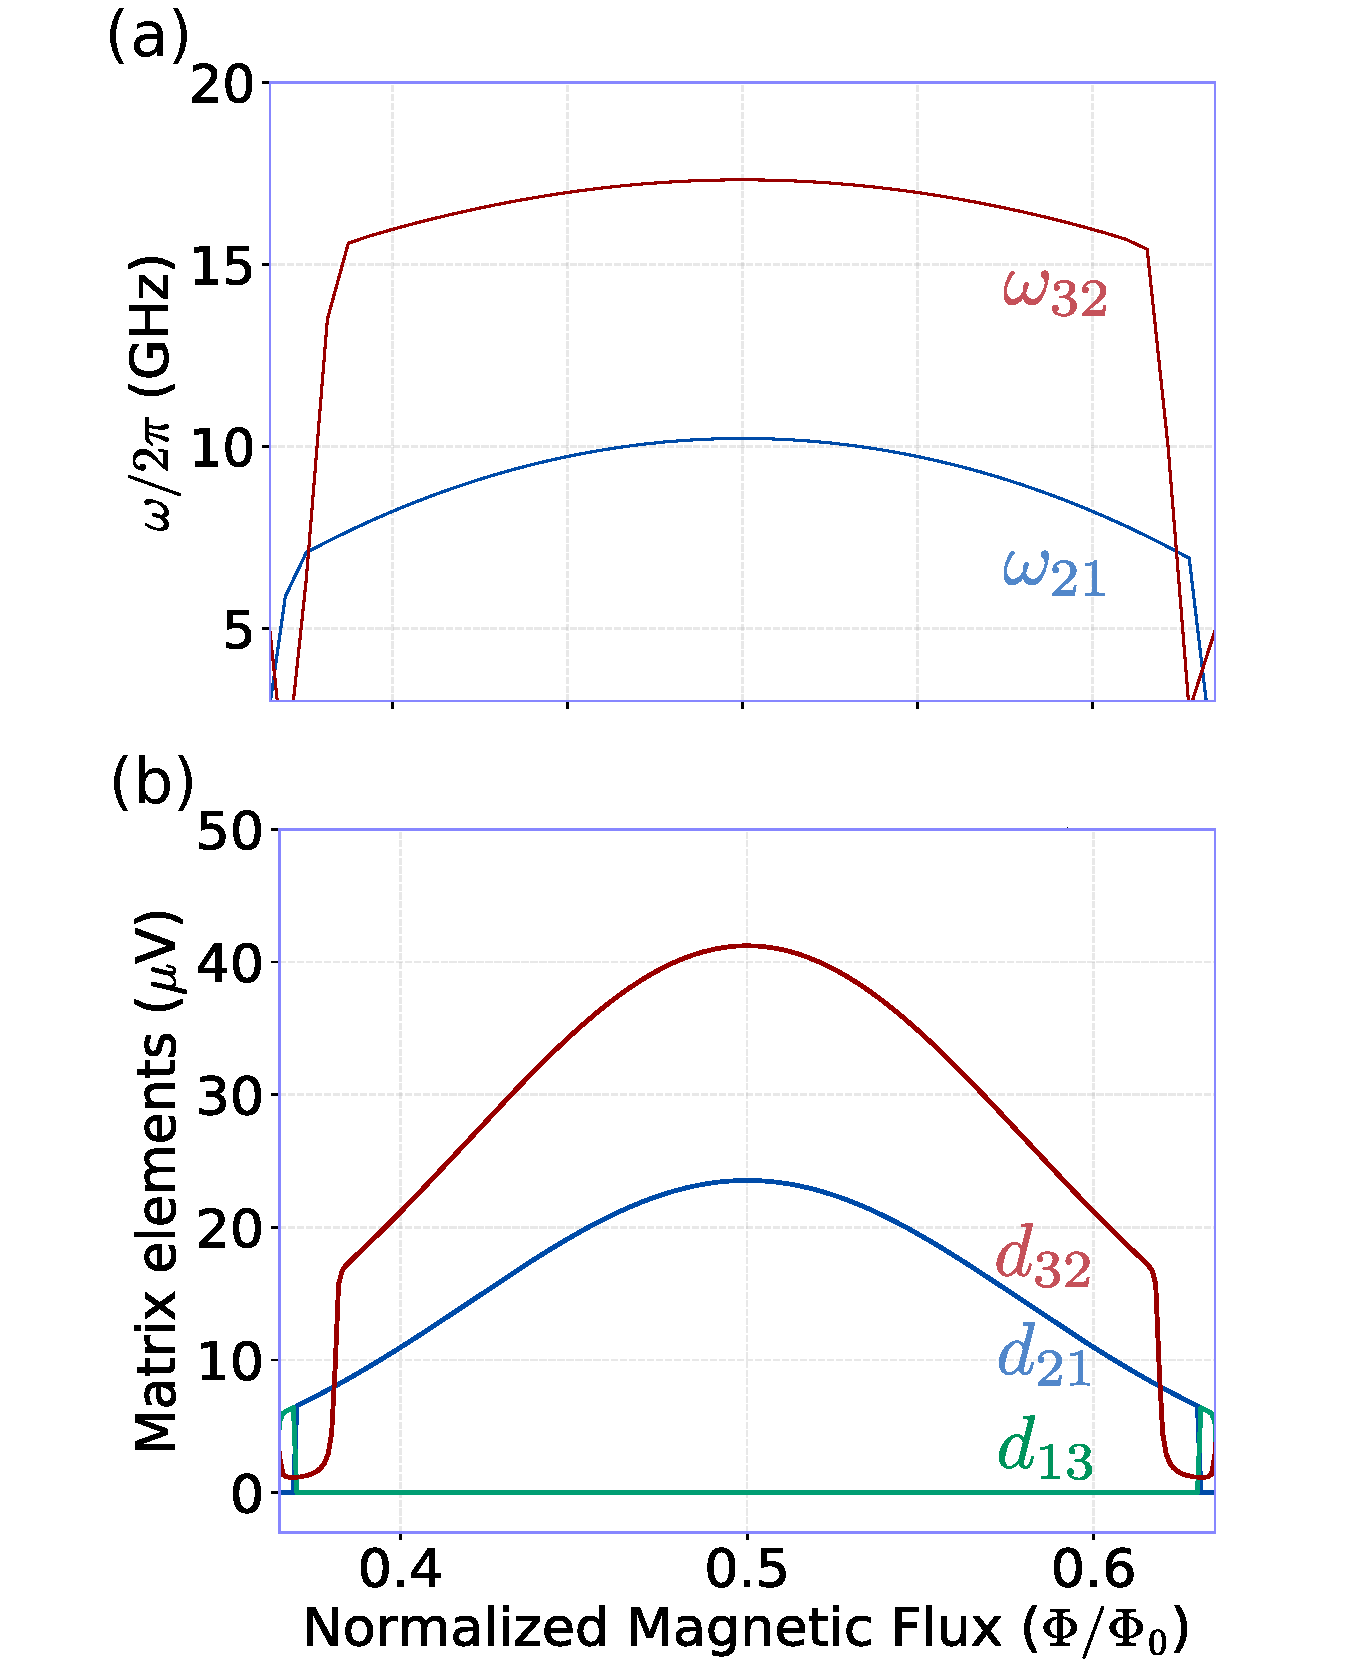
\includegraphics[width=8cm]{fig3}
  \centering\def\svgwidth{8cm}\import{images_inkscape/}{fig3.pdf_tex}
  \caption{\small \textbf{Experimental spectra, circles, and  simulation, solid lines, of the
      twin  qubit:}   Shown  are   the  transition   frequencies  $   \omega_{21}  $   (blue)  and
    $ \omega_{32}$ (red).  Asymmetry  in the flux penetrating the left and  right loops results in
    the  gradual   change  of   transition  frequencies   with  every   $  \Phi_{0}   $  period:
    $\omega_{21}$ creeps  up, while $\omega_{32}$ creeps  down, breaking the usual  periodicity of flux
    qubits.  \label{fig:experiment}}
\end{figure}
 
An  important qubit  parameter is  the curvature  at the  turning points  in the
energy  spectrum, at  the operation  point  of the  qubit.  A  low curvature  is
desirable, to  make the  qubit less  sensitive to  external flux  changes, which
would  improve  decoherence  time.   At   the  twin  qubits'  degeneracy  points
$      \Phi     =      n\Phi_0,     n\in\mathbb{Z}      $,     the      curvature     is
$   (-550\pm10)\,\text{GHz}/\Phi_0^2  $.    It   is   substantially  smaller   than
$  13\times  10^4$ $  \text{GHz}/\Phi_0^2$  on  the  4-JJ flux  qubit  \cite{stern2014},
$   8.4  \times   10^4\,   \text{GHz}/\Phi_0^2$  \cite{zhu2010}   and   $  37\times   10^{4}$
$ \text{GHz}/\Phi_0^2$  \cite{gustavsson2012} on the 3-JJ  flux qubits demonstrated
recently.  However,  the decoherence time  of $  = \iunit{42}{ns} $,  taken with
Rabi  oscillation   \cite{Bylander2011,Ithier2005,Martinis2003}  was  relatively
short, see  Fig.~\ref{fig:rabi}.  We attribute  this to poisoning of  the sample
with  the infrared  radiation, and  the  coupling two-level  oscillators in  the
substrate, owing to the simplified technology used in the qubit's fabrication.

\begin{figure}[h]
  % \includegraphics[width=8cm]{fig5}
  \centering\def\svgwidth{8cm}\import{images_inkscape/}{fig5.pdf_tex}
  \caption{\textbf{Rabi oscillations:}  taken at  the degeneracy point  by driving  the qubit
    with resonant microwaves pulses for fixed time periods, $ \Delta t $.  The decoherence time of
    $   \tau_{\text{dec}}  =   \iunit{42}{ns}  $   is   extracted  from   the  decay   envelope,
    $ e^{-\Delta t/\tau_{\text{dec}}} $, of the the oscillations. \label{fig:rabi}}
\end{figure}
  % Despite the twin qubit have a much the decoherence time
  % in our qubits was
  % relatively small This improved robustness to flux noise
  % is matched by a
  % decoherence time of , extracted from Rabi oscillations
  % in Fig.~\ref{fig:rabi}
  % \cite{rabi}.

%%% Local Variables:
%%% mode: latex
%%% TeX-master: "../dipole_ilya_paper"
%%% End:
